\section{Implémentation C++}

Il n'est pas clair quelle est la forme de l'ensemble de point qui mènera au pire temps de réveil. Cependant, on peut conjecturer que pour le cas pair, il s'agirait d'une répartition uniforme des points sur le cercle et c'est dans ce but que l'on a étudié selon divers algorithmes le temps de réveil du cas "uniforme" à $n$ robots que l'on appelera $\beta_n$.

En utilisant nos algorithmes afin de tracer des approximations de $\beta_n$, on a pu émettre une conjecture indiquant que $\beta_{2n}$ serait décroissante. Cela serait un pas en avant dans la recherche pour montrer que $\alpha_4$ est bien le maximum strict.

Pour tenter de s'assurer de la véracité de ces formules, il est d'abord intéressant de la tester pour divers valeurs de $n$. Mon travail a donc été ici la réimplémentation en C++ d'algorithmes python afin de les accélérer et en particulier pour le cas où les points sont répartis uniformément dans le cercle.

\subsection{Premier algorithme "Segment"}

\large{principe de l'algorithme} il se positionne sur un point de la forme convexe, et choisi un autre point qui coupera alors le polygone en deux parties, On envoi alors un robot pour chacune de ces parties qui s'occuperont récursivement de leurs propres polygones.
Il est important de noter que l'on utilise un cache pour introduire de la programmation dynamique et réduire la complexité.

Segment est un algorithme qui a été créé pour travailler sur le cas général dans l'espoir d'obtenir un bon algorithme polynomial pour le résoudre. Le problème était NP-dur, cet algorithme ne permet en effet pas de résoudre le cas général et manque des solutions. Cyril Gavoille a tout de même prouvé qu'il existe un ordre d'entrée des points permettant à segment de donner la solution optimale. Cependant, étant donné qu'il existe $n!$ solutions, cela n'est qu'une observation.
Dans le cas Convexe, on aurait pu espérer Cependant qu'en donnant les solutions dans l'ordre standard on puisse obtenir une solution optimale. En effet, Le cas où les points sont en position convexe laisse une question ouverte sur son appartenance à $P$. 

il est important d'observer que dans le cas convexe avec l'ordre dans le sens des aiguilles d'une montre de la forme convexe, la solution obtenue présente des arêtes qui ne s'intersectent pas, on dit que cette solution est planaire. 

Dans le cadre d'un cercle où les points sont répartis uniformément, une optimisation excellente consiste à introduire une certaine subjectivité, un duo de robot sur un point n'aura pour environnement de travail qu'un segment défini par sa longueur à gauche et à droite de lui. Il n'existe alors que $n^2$ possibilités. On obtient alors un algorithme polynomial, rapide pour résoudre les $\beta_n$. 

Enfin, c'est ce qu'il aurait été possible de dire si segment permettait de donner les solutions optimales. Malheureusement, cela n'a pas été prouvé et dans le cas plus général convexe, on observe des solutions optimales non planaires et donc automatiquement, segment n'est pas optimal, en voici un exemple:

\begin{figure}[h!]
  \centering
  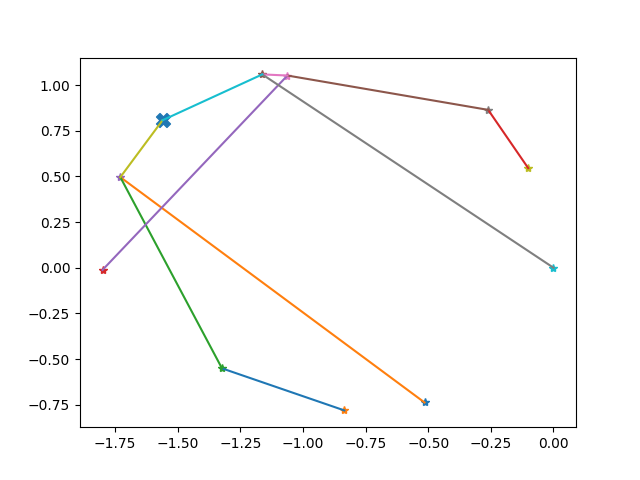
\includegraphics[scale=0.5]{opt_non_plan}
  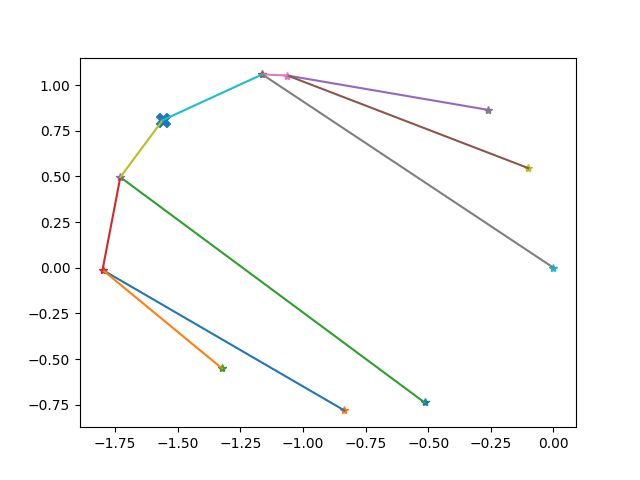
\includegraphics[scale=0.5]{seg_non_plan}
  \caption{Non optimalité de Segment}
  \label{fig:segopt}
\end{figure}

On a à gauche la solution optimale présentant un croisement, exploitant que la branche à gauche est plus courte que celle de droite tandis que sur l'image de droite, on trouve la meilleure solution planaire possible, soit celle donnée par segment. On voit donc bien que segment ne résout pas complètement le cas convexe mais l'approxime.

Ma contribution sur ce sujet aura été l'implémentation et l'optimisation en C++ qui aura ainsi permis d'aller explorer la position uniforme jusqu'à $n = 1000$ sans prendre trop de temps. Il reste encore ouvert si Segment du cas convexe permet de résoudre le cas uniforme et cela forme une nouvelle conjecture.

\subsection{Brute force}

Comme son nom l'indique, cet algorithme cherche à tester toutes les solutions possibles afin de trouver la meilleure possible. En utilisant un cache, il est possible de montrer que cet algorithme est dans le cas général en $\frac{3^n}{\sqrt{n}}$. Avant mon arrivée, pour calculer le temps optimal pour le cas circulaire à $n = 17$ points, il fallait à un bon ordinateur 5 minutes et 17 secondes rendant très compliqué voir impossible d'aller plus loin et donc de vérifier nos conjectures qui ne deviennent ambigües qu'à $n$ grand.

Dans l'objectif de pouvoir aller plus loin dans l'analyse des $\beta_n$. J'ai également réimplémenter l'algorithme brute force en C++ permettant alors de calculer le cas $n = 17$ en 1 minute et 18 seconde, un progrès significatif surtout que ce temps est obtenu sur un pc bien moins bon.
Ironiquement, la plus grand optimisation aura été de rajouter "-O3" à la commande de compilation pour laisser le compilateur tout optimiser à sa façon, utilisant des fonctions avancées du processeur. On descend alors à 18 secondes.
Pour que cela soit possible, que le compilateur puisse optimiser autant, il faut noter qu'une grande amélioration aura été de représenter les ensembles de points présents en grande quantité dans le code par une classe spéciale basée sur un entier 64 bit où un 1 en position i signifie que i est dans l'ensemble. Un tel objet fonctionne bien car on sait que brute force ne pourra jamais atteindre $n = 64$ et donc qu'on aura jamais plus de 64 points, soit le nombre de bit dans un entier 64 bits. Par ce biais, il a été possible d'optimiser les opérations de création des ensembles, et d'en réduire le coût mais surtout de simplifier pour l'ordinateur l'étape suivante...

En effet, jusque là, les optimisations marchent dans le cas général, et n'utilisent absolument pas la structure de polygone régulier du problème. Pour représenter parfaitement le polygone régulier, on peut penser aux isométries, les opérations que j'ai nommé "miroir" de symétrie axiale et "shift" de rotation centrale. l'ensemble des rotations et d'une seule de ces symétries axiale engendre tout le groupe des isométries du polygone régulier. 
Si l'on cherche à traduire cela avec notre groupe de bits représentant un ensemble, cela revient à dire qu'en déplacant les bits de droite à gauche et inversement (ainsi que le point de départ des robots) donne exactement la même solution à "shift" pres.
Alors, pour représenter cela, on fait en sorte le point de départ des robots soit toujours 0 afin que toutes les solutions qui soient un décalage d'une autre se reconnaissent comme étant les mêmes. Cela mène à une solution nommée "shift invariant" réduisant alors le temps d'exécution pour $n = 17$ à 9.5 secondes. Il est à noter que la rotation des bits se fait très bien avec des opérations binaires simples et donc est une opération au goût du compilateur.
Il reste alors la dernière optimisation, celle du miroir. Sachant avec l'optimisation précedente que le point de départ des robots est en 0, l'opération miroir revient à effectuer un effet miroir sur les bits sauf le bit en 0 qui reste le même. 
Malheureusement, il n'existe aucune opération binaire simple permettant d'effectuer un effet miroir sur les bits et j'ai donc du utiliser un "bit hack" qui effectue un algorithme court pour résoudre le problème en diviser pour régner.

\begin{verbatim}
	short bits = 64;
    unsigned long long mask = ~(0llu);

    while (bits >>= 1) {
        mask ^= mask << (bits);
        n = (n & ~mask) >> bits | (n & mask) << bits;
    }
\end{verbatim}

Cet algorithme fonctionne en inversant d'abord les groupes de 32 bits, puis les groupes de 16 bits puis ... à l'aide d'un masque.

Une fois cela fait, pour faire en sorte que les opérations soient invariantes par "mirror", je trompe le cache en lui indiquant de considérer égaux des entiers non seulement si leurs ensembles sont égaux mais aussi si le miroir est égal à l'autre entier. Et cela descend le temps d'execution pour $n = 17$ à 4.5 secondes.
Grâce à ces optimisations on sera descendu de 5 minutes et 17 secondes à 4.5 secondes.

\subsection{Mon propre algorithme}

En arrivant à mon stage, je suis arrivé avec un algorithme en tête cherchant à résoudre le problème dans le cas convexe, un algorithme se situant entre le brute force et segment. Malheureusement, il n'est pas polynomial, et il ne résout pas non plus le problème. Cette approche reste sur l'approche consistant à choisir des sous ensembles pour nos robots sauf que là où segment coupe en deux segments et brute force choisi tous les sous groupes de travail de possible, ce nouvel algorithme sélectionne des ensembles de points dont les enveloppes convexes sont disjointes. Cela revient à tracer une droite sur un cercle pour couper le cercle en deux morceaux. Segment est ainsi le cas particulier où le point de départ est forcement sur la droite de coupure et présente donc n possibilités là où mon algorithme présente $n^2$ explorations récursives. L'analyse de la complexité d'un tel algorithme toujours avec cache est extrêmement compliquée et c'est seulement expérimentalement qu'on observe la nature exponentielle du nombre d'étape. Cet algorithme permet de trouver des solutions non planaires ce qui n'était pas le cas de segment. Malheureusement, \ref{fig:segopt} permet de conclure à la non optimalité de cet algorithme. Pour trouver ce contre-exemple, il a d'ailleurs fallu que j'implémente l'algorithme et que je l'optimise au même titre que l'algorithme de brute force afin de le faire tourner jusqu'à trouver un résultat où le brute force est meilleur que mon algorithme. En python, il me fallait 720 secondes pour un seul test alors qu'en c++, j'en faisais plusieurs par seconde grâce à une nouvelle implémentation.
En dépit de ses défauts, un tel algorithme reste plus rapide que l'algorithme de brute force en effet, après y avoir ajouté exactement les nouvelles améliorations de brute force pour le cas uniforme, on obtient l'execution de cet algorithme pour $n = 17$ en 0.05 secondes ce qui permet enfin de viser des n plus grands. avec mon faible ordinateur, n = 32 n'était alors plus un rêve.

\subsection{Conjectures}

Ainsi, on possède des algorithmes plus rapides pour explorer les conjectures plus profondément. Premièrement, pourquoi cette valeur de n = 32 était importante. Il était observé par Cyril Gavoille qu'en utilisant segment on obtenait $\beta_{60} < \beta_{62}$ ce qui cassait la conjecture de décroissance de $\beta_{2n}$, on se demandait si alors en réalité, la conjecture était vraie, mais que les solutions dans le cas uniforme devenaient non planaires, chose qui était difficilement envisageable avant. On m'avait alors assigné la tâche d'atteindre avec des algorithmes un peu plus puissants cette valeur $n = 62$. En supposant la symétrie de part et d'autre du cercle, on pouvait essayer d'utiliser un puissant algorithme pour $n = 62$ avec 32 points et espérer d'obtenir une meilleure solution. Cependant, partir avec la moitié des points utilise moins les optimisations de cache que partir avec tous les points, faisant que le temps de calcul de $n = 32$ était au final bien plus court que celui de $n = 62$. En réalité, avec mon algorithme et en supposant la symétrie, je n'ai pas pu dépasser $n = 52$. Sans nouvelles pistes d'améliorations, je dû donc abandonner cet espoir d'atteindre $n = 62$.

Et c'est alors en voulant dessiner un graphe des $\beta_{2n}$ (avec segment) pour le rapport de stage afin de justifier la conjecture que j'ai remarqué quelque chose... de surprenant.

\begin{figure}[h!]
  \centering
  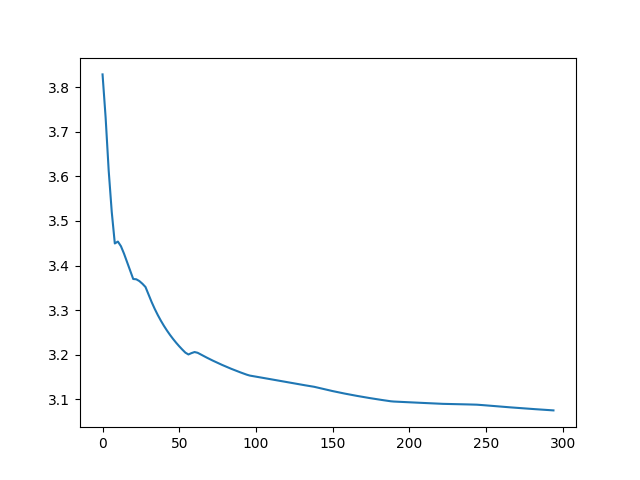
\includegraphics[scale=0.5]{beta_2n1}
  \caption{$\beta_{2n}$}
  \label{fig:beta2n1}
\end{figure}

On observe bel et bien le petit saut en $n = 62$
cependant... on observe deux pics avant cela, un pic en $n = 14$ et un faux pic en $n = 24$ qui en réalité ne casse pas la conjecture. Mais ce qui est important, c'est qu'on observe une exception bien avant $n = 62$! or pour $n = 14$ on peut aisément faire le calcul avec l'algorithme de brute force. Et l'algorithme de brute force et segment coïncident pour $n \leq 17$
On alors bien que la conjecture était fausse. On pourrait alors imaginer de nouvelles conjectures, en particulier sur où sont les exceptions. Il a d'abord été proposé par mon encadrant des formules basées sur $4^n$ car 4 est un maximum, 16 est proche d'une exception et 64 est un maximum local. Cependant, n'ayant aucune autre exception pour $n \leq 300$ la série se casse. Peut être peut on alors se dire qu'il s'agissait d'exceptions et qu'il n'y en a plus après, et pourtant...

\begin{figure}[h!]
  \centering
  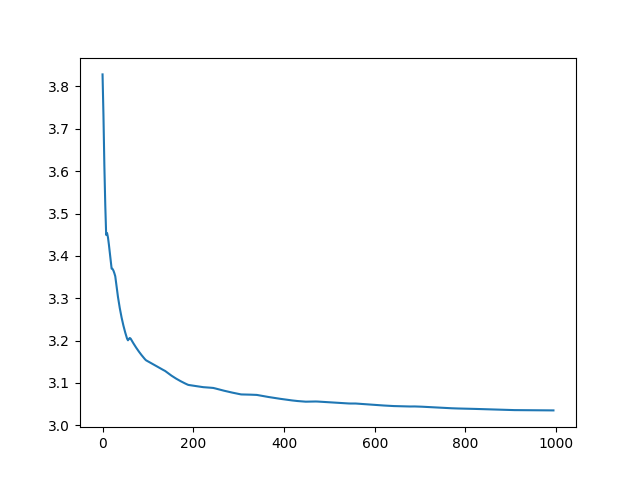
\includegraphics[scale=0.5]{beta_2n2}
  \caption{$\beta_{2n}$ jusqu'à $n = 500$}
  \label{fig:beta2n2}
\end{figure}

On observe rien de plus sur cette figure, elle semble lisse après les exceptions et prend désormais en compte les $n \leq 1000$ ce qui va bien plus loin, mais.. en cherchant avec python des maximums et des minimums, voici ce que l'on obtient:

\begin{verbatim}
local maximum:  4
local minimum:  12
local maximum:  14
local minimum:  60
local maximum:  64
local minimum:  450
local maximum:  474
local maximum:  476
local minimum:  550
local maximum:  560
local minimum:  678
local maximum:  688
local minimum:  802
local minimum:  804
local maximum:  806
\end{verbatim}

On observe nos anciens pics mais on observe surtout de nouveaux pics qui ont l'air complètement chaotiques. Cet air chaotique est probablement donné par des solutions d'équations trigonométrique mais cela montre surtout qu'il n'y a pas d'espoir de trouver des solutions simples, que nos conjectures sont justes fausses et donc que ce que certains chercheurs s'acharnaient à vouloir montrer ne pouvaient être faits car cela n'était tout simplement pas vrai... Voici quelque part ma contribution dans le domaine des conjectures. Et tout cela grâce à des algorithmes optimisés comme possible.